\section{Implementation} %Control Approach}
\label{chap:controlApproach}

The conceptual design elements that are explained in the previous section have been implemented to represent the envisioned framework. This section illustrates how designed concepts are realized in various hardware and software components. 

Physical system components are first introduced to shed light on the experimental facility, localization system and give more details on low level actuator control systems running on the modules. The multi-robot network setup is explained showing how various system components communicate. A object oriented Matlab software-framework been developed aimed to be reusable and intererable for other multi-vessel experiments within RAS. This framework, its structure, relation between classes, and means of implementing the designed control approach are explained in section \ref{sec:controlSoftware}.

Throughout developments many iterative changes were made to the system, of which two facets are discussed in section \ref{AdjustmentsAfterTests} starting with the process of tuning control gains and secondly an improvement of the assembly protocol using normal forces between modules to aid connectors reaching area of acceptance. 

Behaviors and responses of the system in development are occasionaly shown to support design choices. Behavior of the system in final stage of development is shown and evaluated in the next chapter. 

\subsection{System Components}
\label{imp:syscomponents}
The implemented control system consists of three key components
\begin{itemize}
	\item An optical tracking system for module localization.
	\item A computer that executes the control protocol and distributes generated tasks to the entire fleet.
	\item A set of Delfia-1* modules
\end{itemize}

This section provides details on the experimental setup of the optical tracking system and modules. Functionality of the control software is discussed in a separate section (\ref{sec:controlSoftware}). 

%\subsubsection{Experimental facility and Optical tracking system}
The experimental setup is designed to operate in the towing tank facility of section Maritime and Transport Technology (section MTT) in the faculty of Mechanical, Maritime and Materials Engineering (Faculty 3ME). One of such tanks is equipped with an optical sensing and interpretation system from the brand Optitrack. A 40 meter section of the tank is covered by cameras. Optitrack's motion capture software supports defining a set of infra-red reflectors as a rigid body. The camera setup was set up to interpret images to estimate state of the defined bodies (modules), and broadcast them on dedicated ROS topics at a frequency of 30hz. 

\begin{figure}[h!]
	\centering
	\captionsetup{justification=centering}
	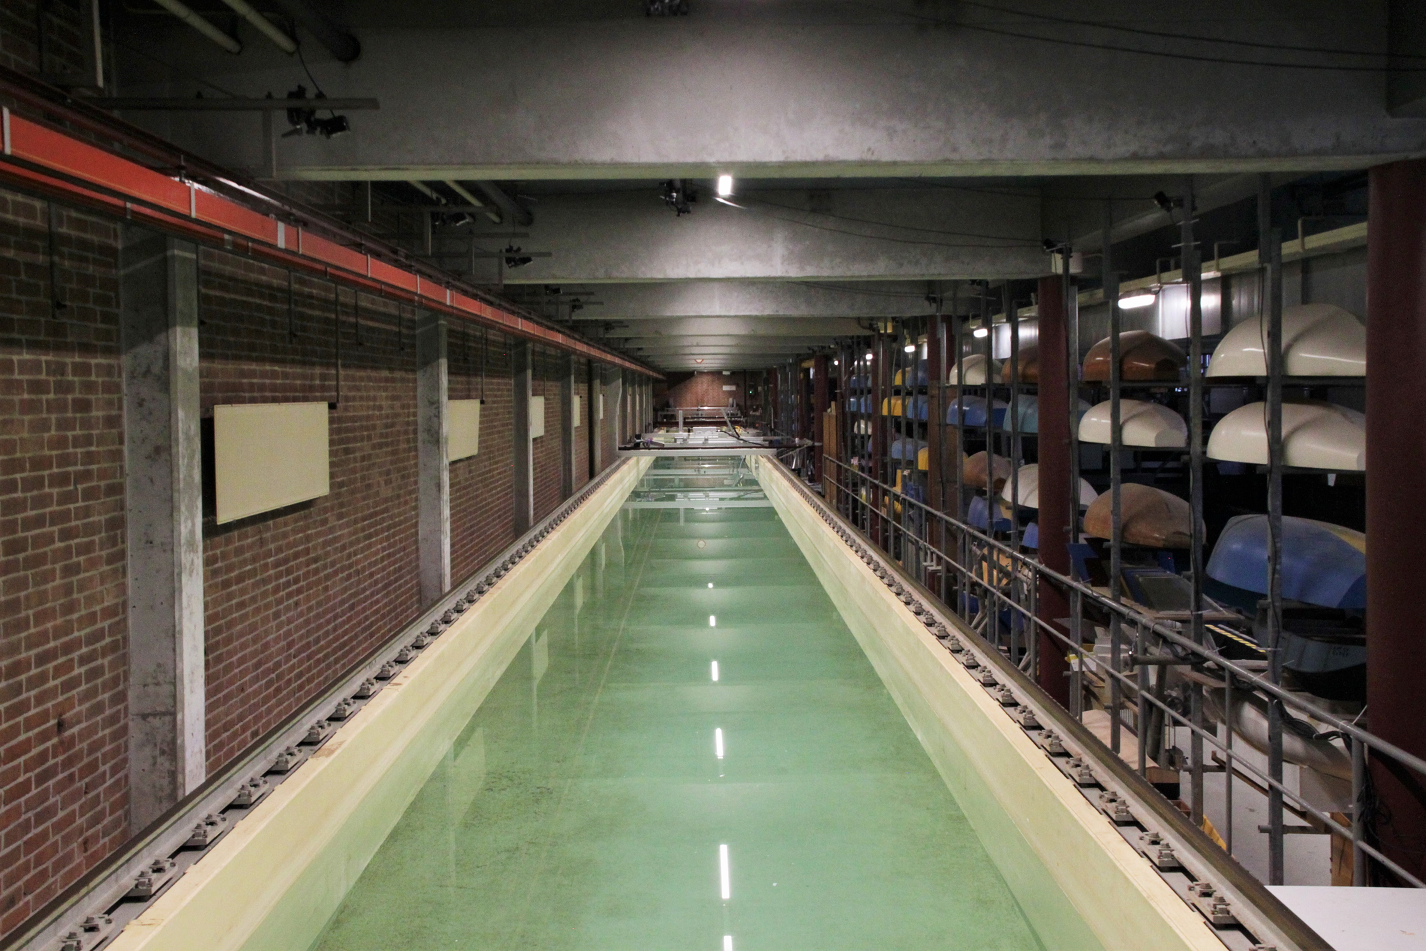
\includegraphics[width=0.9\textwidth]{img/IMG_4805b_downsized}
	\caption{The MTT towing tank facility at 3ME.}
\end{figure}


\begin{figure}[H]
	\centering
	\makebox[\textwidth][c]{
		\begin{minipage}{0.4\textwidth}
			\centering
			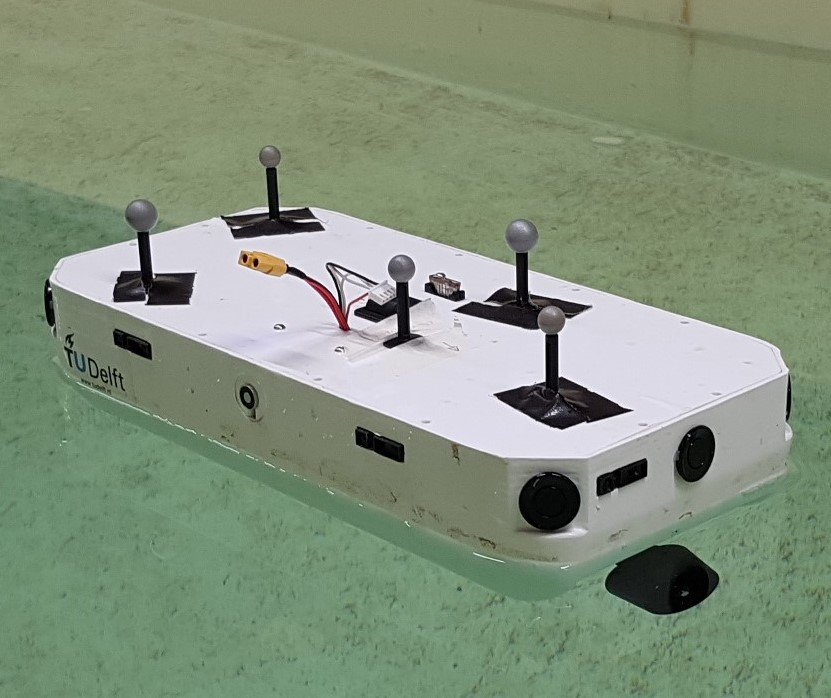
\includegraphics[width=0.95\textwidth]{img/singleDelfiaInfraRedTrackers}
			\caption{Five infra-red reflectors on top of a Delfia-1* module.}
		\end{minipage}\hfill
		\begin{minipage}{0.55\textwidth}
			\centering
			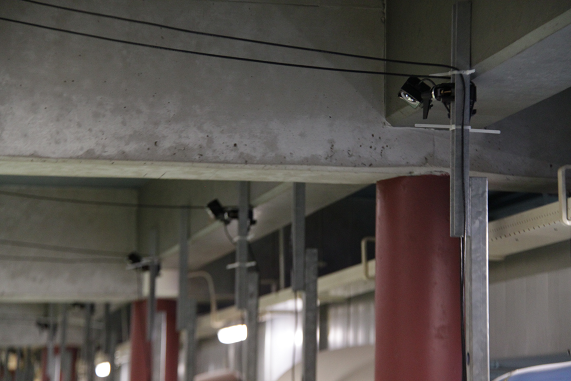
\includegraphics[width=0.95\textwidth]{img/IMG_4810_downsized}
			\caption{Motion tracking cameras mounted along the experimental setup.}
		\end{minipage}
	}
\end{figure}

\begin{figure}[H]
	\centering
	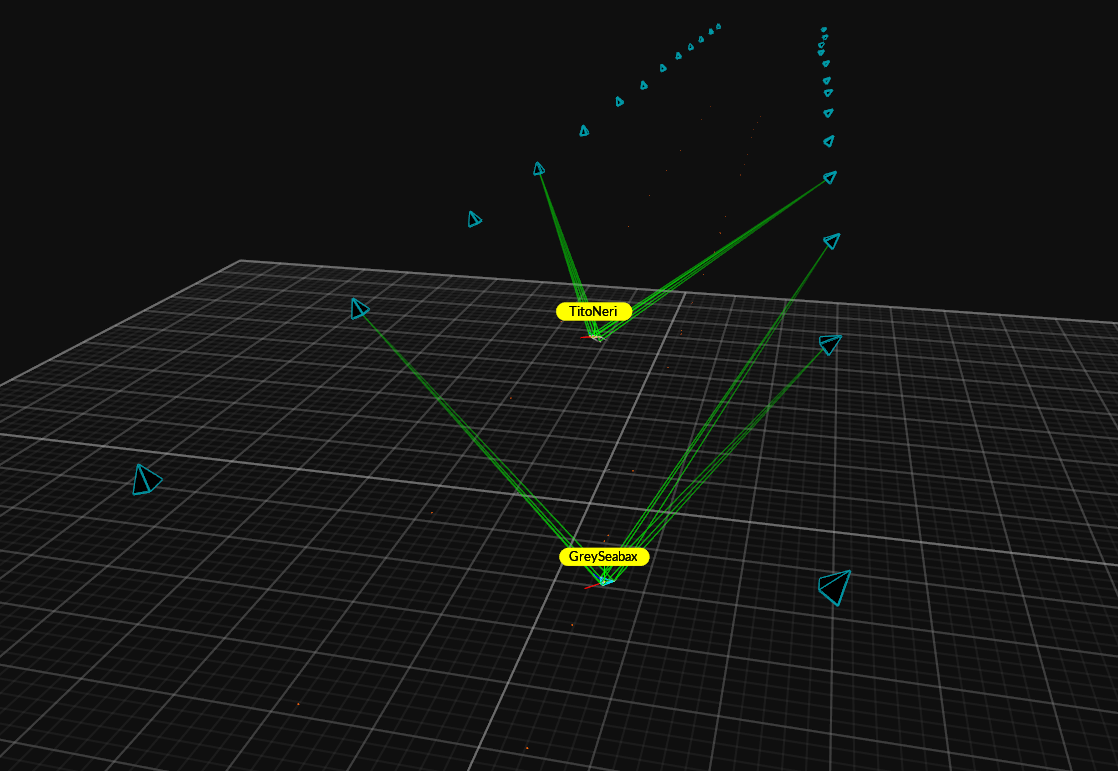
\includegraphics[width=0.7\textwidth]{OptitrackRays}
	\caption{Optitrack motion tracking with the towing tank setup, showing two deployed vessels. Green lines depict rays of reflectors that are succesfully being tracked}
\end{figure}


%\subsubsection{Delfia-1* Modules}
The Delfia-1* vessel (also refferd to as 'Delfia') is a model scale, electrically powered ship, equipped with two 360 degree rotatable azimuth thrusters. There are a total of four main actuators that are controlled by an on board system, referred to as the 'low-level control system'. The two azimuth thrusters are identical, and both have their orientation and propeller speed managed by a single microprocessor of the open-source Arduino project. Control of propeller speed and thruster angle is done with different hardware components, yet both rely on similar PID feedback control principles. Figure \ref{DelfiaDOF} illustrates the states that the low level control system needs to manage for one thruster. 

\begin{figure}[h!]
	\centering
	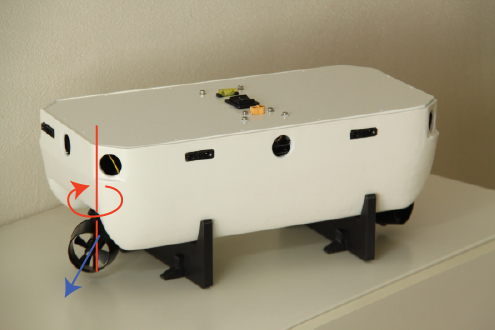
\includegraphics[width=0.7\textwidth]{IMG_4564}
	\caption{Degrees of freedom of one azimuth thruster. Each thruster (front and back) needs its direction (red) and propeller speed (blue) controlled.}
	\label{DelfiaDOF}
\end{figure}
All decisions for the low level control system are made on the on board microprocessor. This controller responds to actuator reference commands via USB serial port connection. Connectivity of the low level control system with other elements in the network is done through a Raspberry-Pi, as illustrated in figure \ref{delfiaConnectionNW}. The Raspberry-pi is the connecting element to the ROS network (via wifi) and the Arduino (via USB serial protocol). Other solutions exist that provide similar connectivity, yet a Raspberry-pi has some processing power which allows distribution of some, or all control tasks in future projects. 

\begin{figure}[H]
	\centering
	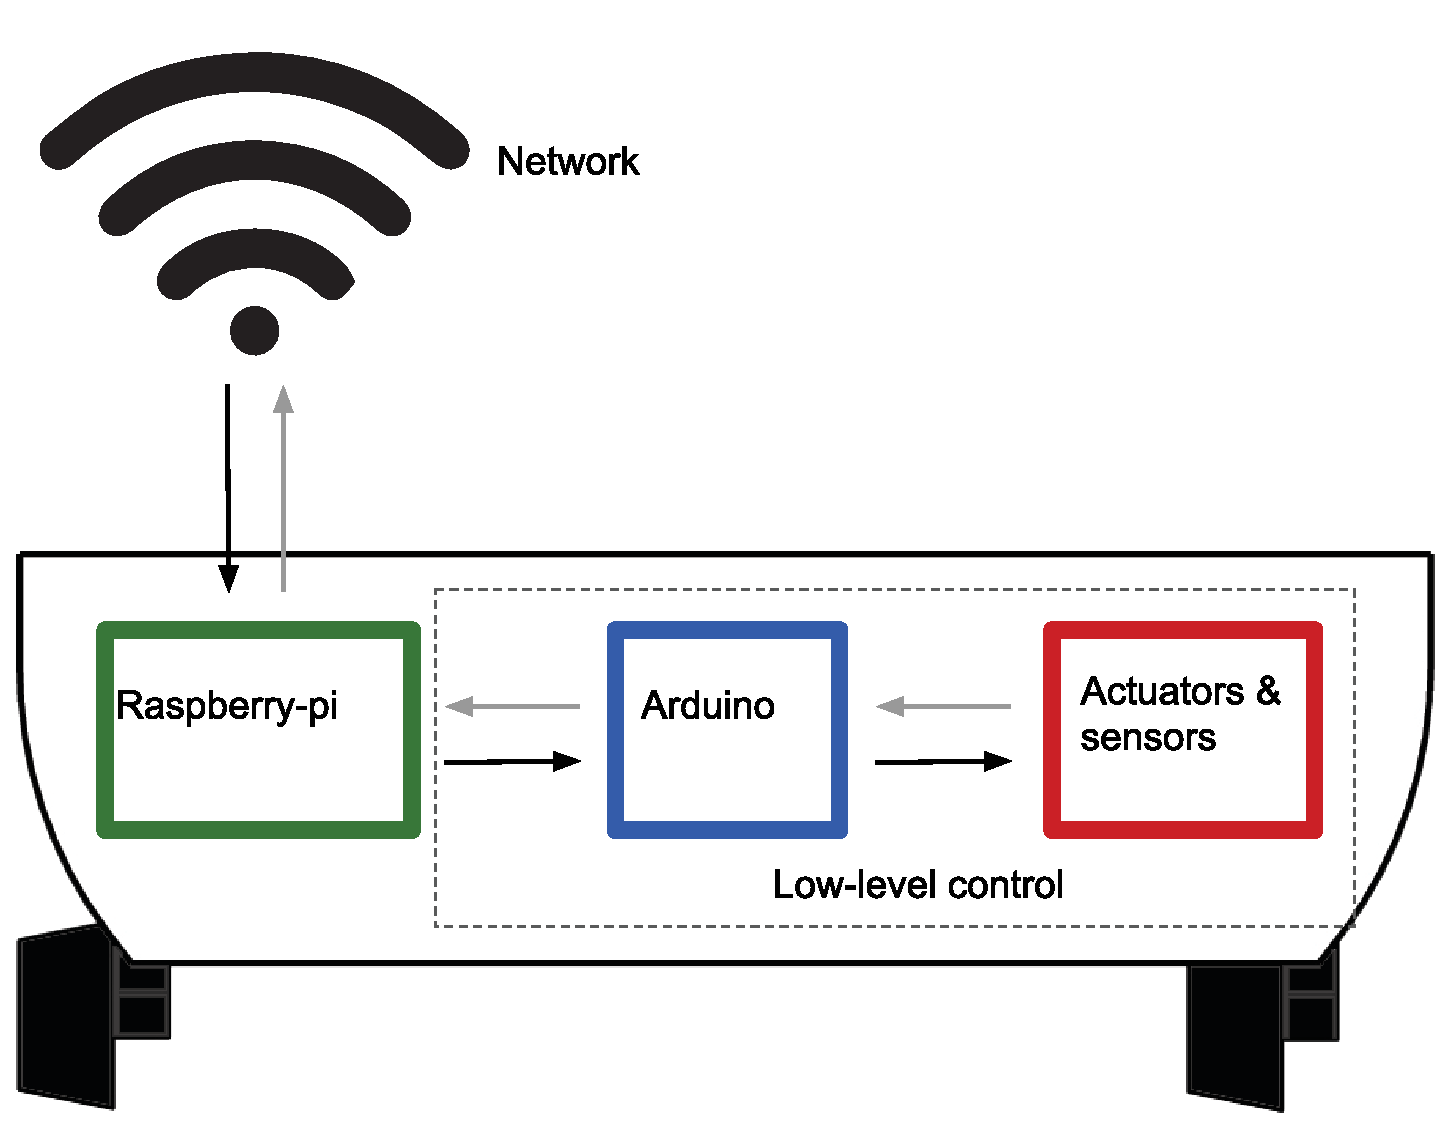
\includegraphics[width=0.5\textwidth]{DelfiaNetworkSchematicLowLvl1}
	\caption{The interaction of the Delfia's low level control system with on board computer (Raspberry-pi) and the vessel network.}
	\label{delfiaConnectionNW}
\end{figure}

The propeller is powered with an electrical 12V DC engine, while a sensor signal on speed is created by means of an optical encoder. Figure \ref{DelfiaDriveTrain} shows the propeller drivetrain that can be found above each thruster, and figure \ref{propellerFBLoop} illustrates the feedback loop that controls propeller velocity. 

 \begin{figure}[h!]
	\centering
	\makebox[\textwidth][c]{
		\begin{minipage}{0.45\textwidth}
			\centering
			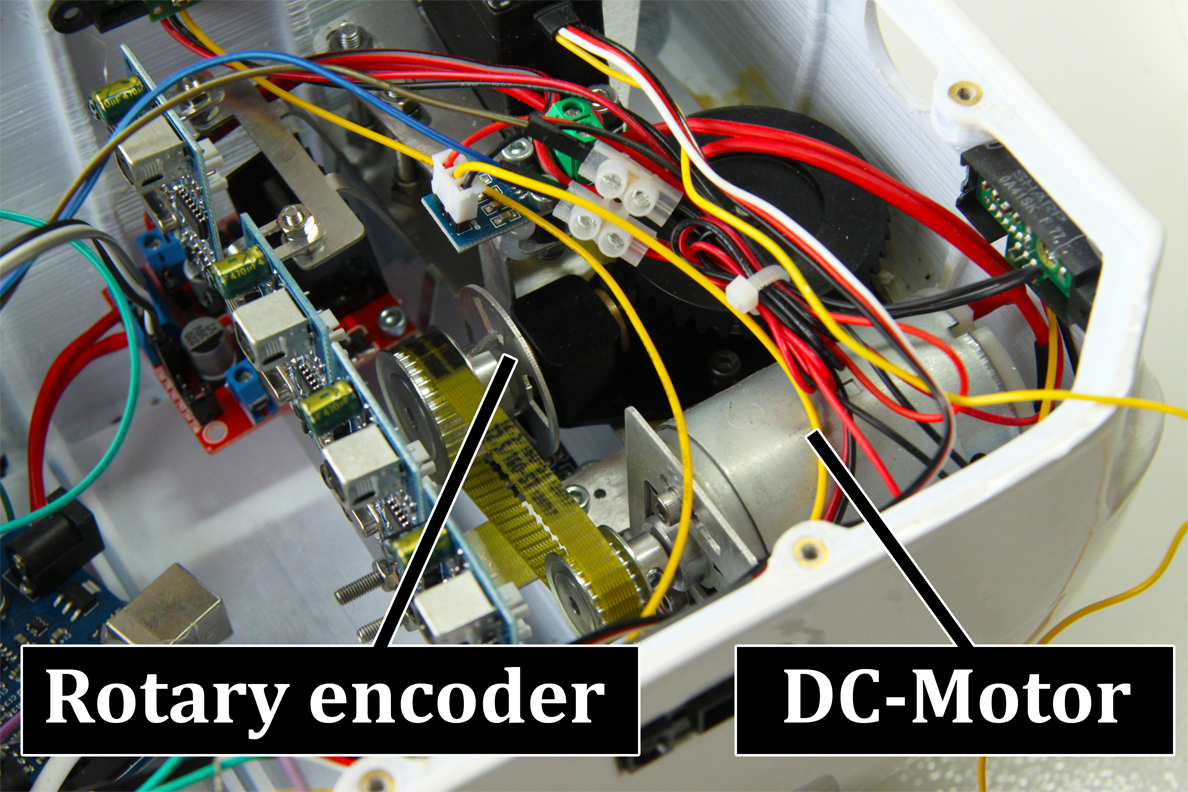
\includegraphics[width=0.95\textwidth]{img/delfiaDriveTrain_edited}
			\caption{The propeller drivetrain. The rotation in the axle of the DC-motor is transferred to the propeller via a belt and gears.}
			\label{DelfiaDriveTrain}
		\end{minipage}\hfill
		\begin{minipage}{0.45\textwidth}
			\centering
			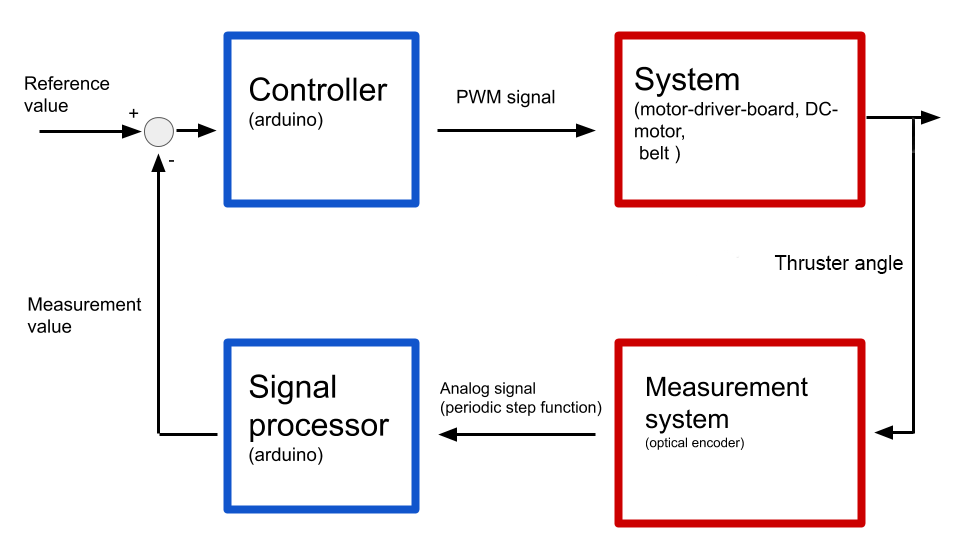
\includegraphics[width=1.1\textwidth]{img/propellerFBLoop}
			\caption{The feedback loop of the low level propeller-speed control system}
			\label{propellerFBLoop}
		\end{minipage}
	}
\end{figure}

Each thruster angle is actuated by a ''Parallax Feedback 360° High-Speed Servo''. Thruster and servo are connected via a rubber cog belt (figure \ref{DelfiaServoTrain}). The servo needs a 50Hz PWM signal as input and uses a hall effect sensor to provide angular position feedback as a 910Hz PWM signal. The feedback loop that controls the thruster angles is as shown in figure \ref{DelfiaServoLoop}.

 \begin{figure}[h!]
	\centering
	\makebox[\textwidth][c]{
		\begin{minipage}{0.45\textwidth}
			\centering
			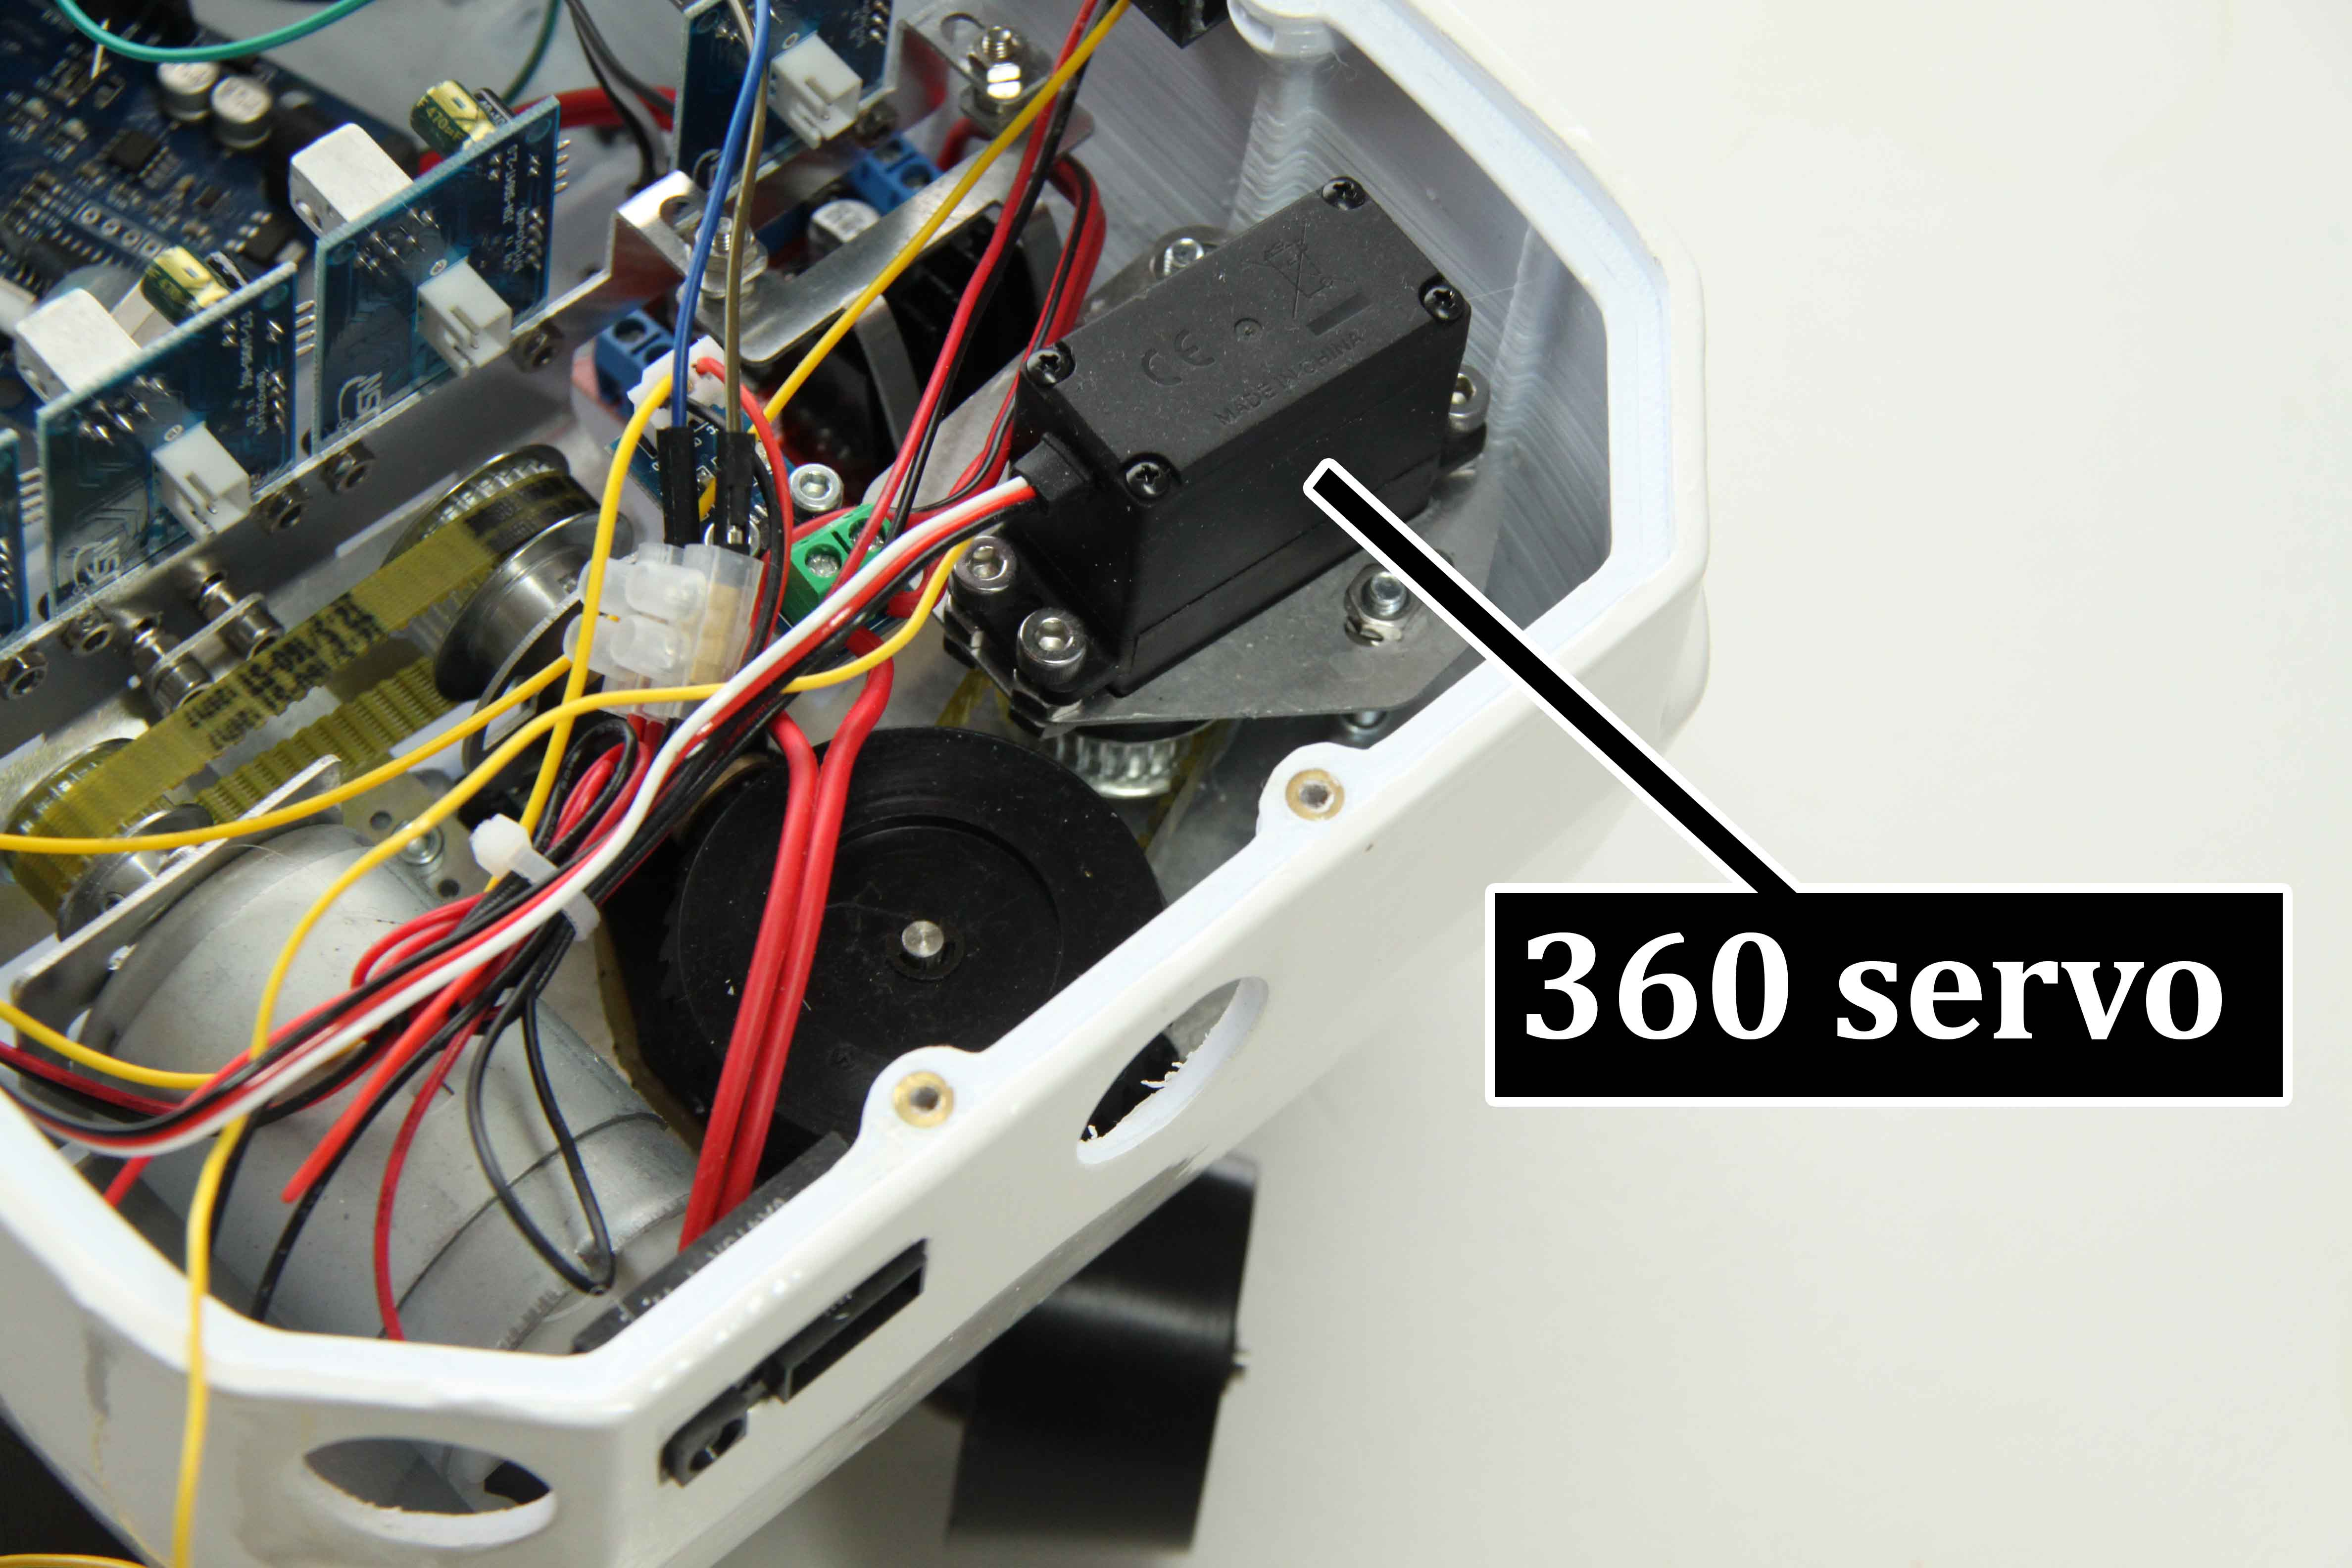
\includegraphics[width=0.95\textwidth]{img/delfiaServo_edited}
			\caption{The propeller drivetrain. The rotation in the axle of the DC-motor is transferred to the propeller via a belt and gears.}
			\label{DelfiaServoTrain}
		\end{minipage}\hfill
		\begin{minipage}{0.45\textwidth}
			\centering
			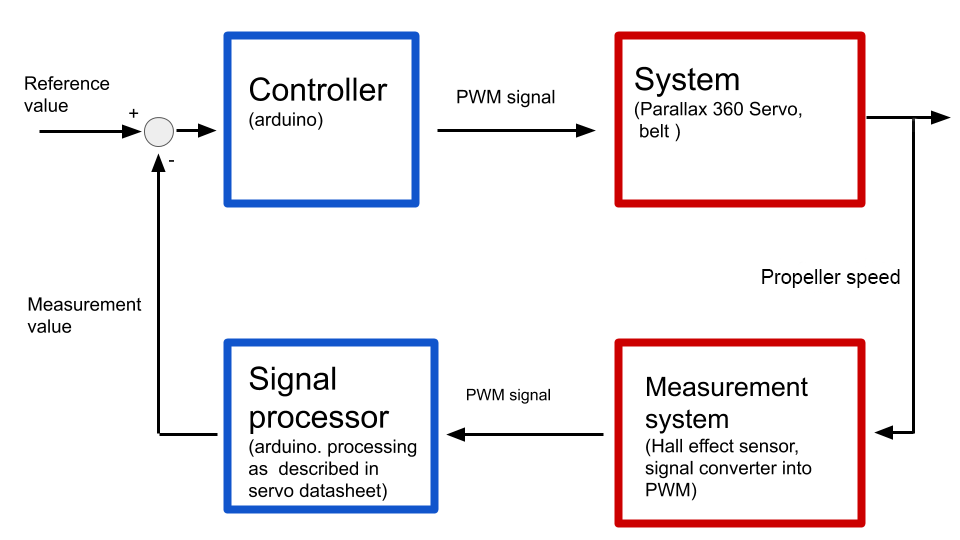
\includegraphics[width=1.1\textwidth]{img/servoFBLoop}
			\caption{The feedback loop of the low level thruster angle control system}
			\label{DelfiaServoLoop}
		\end{minipage}
	}
\end{figure}


Fundamentals of the Delfia-1* low level control system have been developed during a research project \citet{boogmans2020Delfia}, by the same author as this work. Development of hardware and software is described therein, and parameter tuning is done by means of evaluating reference step responses. Characteristic control system behavior is shown in figures \ref{delfiaLowStepProp1} and \ref{delfiaLowStepServ1} for propeller-speed and thruster-angle respectively. Note how the propeller speed signal contains significant fluctuations, of which the majority is considered sensor noise. An optimum trade-off point of signal filtering was found between smoothness and increased latency. High frequency notes in this signal (order of $10^3$hz) that translate to engine control effort will not result in noticable differences of vessel dynamics response, as the  vessel responds in much lower frequencies (order of $10^0$ hz). 

\begin{figure}[H]
	\centering
	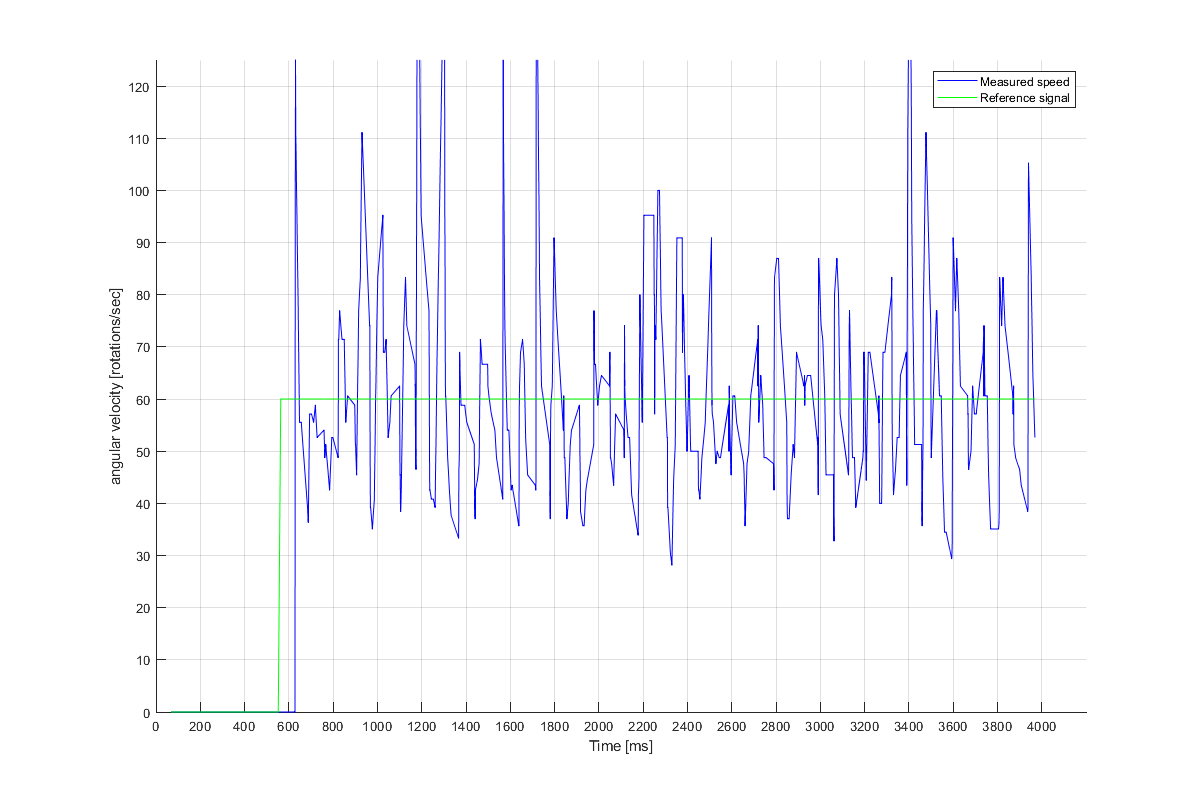
\includegraphics[width=0.85\textwidth]{img/4e-2_2e-2_0_130hz_n=8}
	\caption{Measured signal of a characteristic step-response of the propeller-speed control system. Considerable high frequency notes can be observed, although it oscillates rather well around the reference input.}
	\label{delfiaLowStepProp1}
\end{figure}

\begin{figure}[H]
	\centering
	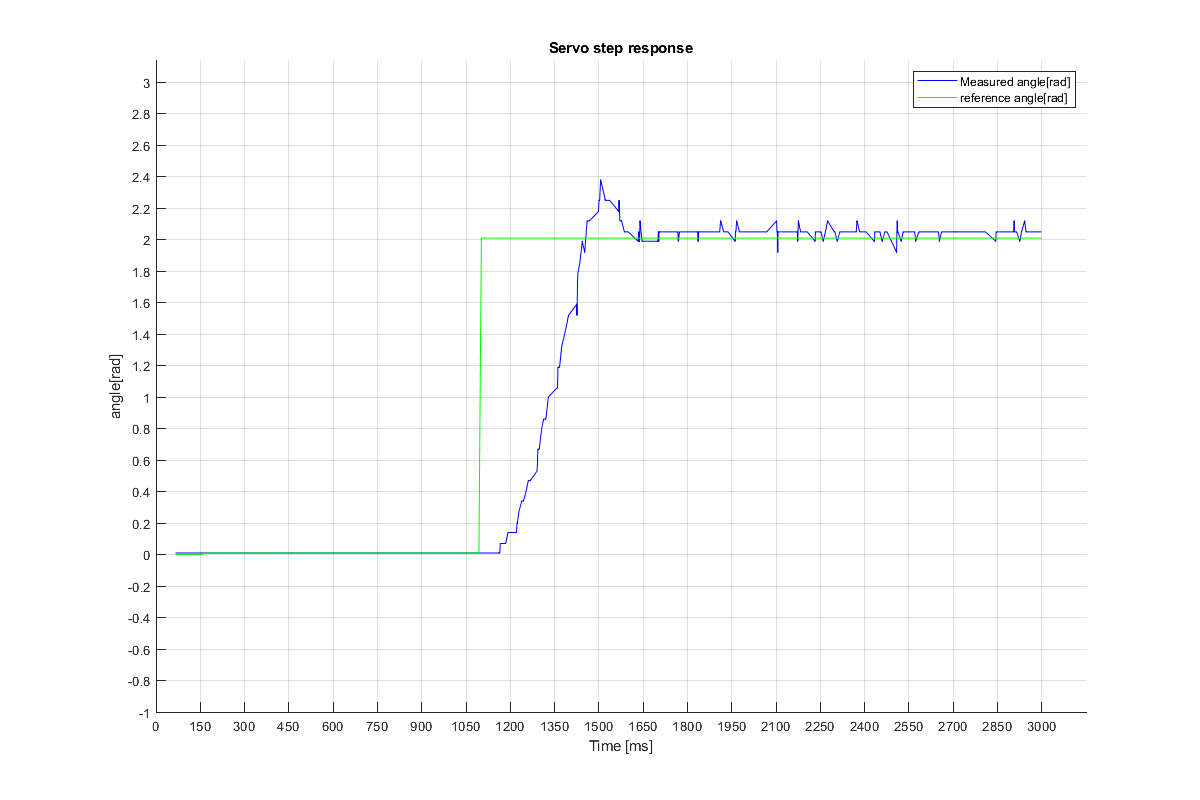
\includegraphics[width=0.85\textwidth]{img/Kp_1e0_Ki_8e-3_Kd_4}
	\caption{Measured signal of a characteristic step-response of the thruster-angle control system.}
	\label{delfiaLowStepServ1}
\end{figure}

It is worth noting that the slope of the servo step response, as shown in figure \ref{delfiaLowStepServ1}, proved quite consistent with more agressive controller gains. Higher proportional or integral gain caused more overshoot, or even instability, without the benefit of a quicker response time. This is considered simply due to the maximum rotation speed of the servo. 


Actuators that connect the modules have been developed and implemented as a set of active magnets, or solenoids, shown in figure \ref{fig:solenoidsMF} and \ref{fig:solenoids}. Models are available in various lifting capacities, and a $10N$ model that operates at $12V$ was estimated to provide enough force for vessels to remain connected in reasonably expected scenarios. It is powered by the $12V$ micro powergrid from the on-board battery.  Higher powered magnets draw more power, and this variant seemed a good balance at a $1.0W$ power consumption. Mounts for the connectors were developed and fabricated by a 3D printer to fit in existing slots in the Delfia's hull.

At first, connections were implemented where a connection was made between two vessels with connectors of opposite polarity. Magnet connector polarity can be reversed by reversing the potential on coil connectors. This can be automated with, for instance, an H-bridge. Tests proved connector force to be insufficient between connecting solenoids. Attracting forces to a piece of iron did give the desired results, thus connector counterparts were lathed to size. Available 3D printers proved to have tolerances sufficient such that connector parts, both magnet and piece of iron, were made to stay in the mouts by using a press. 


 \begin{figure}[H]
	\centering
	\makebox[\textwidth][c]{
		\begin{minipage}{0.48\textwidth}
			\centering
			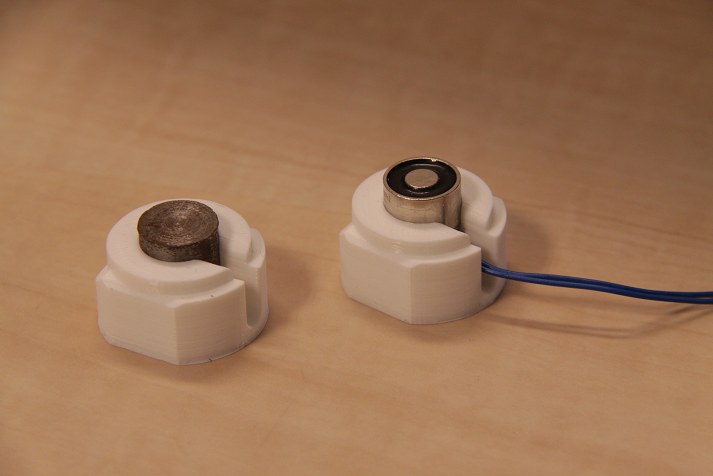
\includegraphics[width=0.95\textwidth]{img/IMG_4812_downsized}
			\caption{An active (right) and passive (left) magnetic connector in a (white) 3D-printed hull mount.}
			\label{fig:solenoidsMF}
		\end{minipage}\hfill
		\begin{minipage}{0.48\textwidth}
			\centering
			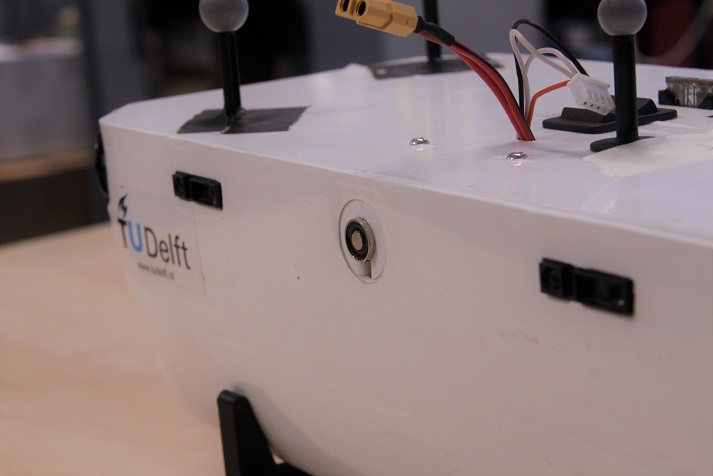
\includegraphics[width=0.95\textwidth]{IMG_4814_downsized}
			\caption{Active magnet mounted in the hull of a Delfia-1* module to connect modules into a rigid platform.}
			\label{fig:solenoids}
		\end{minipage}
	}
\end{figure}

\subsection{Network setup}
The backbone of the communication system is deployment of ROS over an internet network. Vessels connect over WiFi, while shore facilities connect to the network router through ethernet cables. ROS provides various standardized messagetypes to improve interoperability and modularity. Various conventions that are developed throughout this project are intended to serve as a framework for further development and reasearch in the facilities of Researchlab Autonomous Shipping. The proposed standardization includes:
\begin{itemize}
	\item ROS message types for control related signals
	\item Naming convention for control related ROS-topics
	\item IP adress reservations for vessels and other components
\end{itemize}
Table \ref{tab:ROSmsgTypeTable} shows the proposed conventions for communication over ROS in RAS facilities. 

\begin{table}[H]
	\centering
	\begin{tabular}{lll}
	Topic content & Messagetype & Naming convention \\[10pt] \hline
	Vessel position and orientation	&$geometry\_msgs/PoseStamped$ &  $/vrpn\_client\_node/<vesselname>/pose$    \\[10pt]
	
	Vessel Actuation	&   $std\_msgs/Float64MultiArray$     & $/actuation<vesselname>$  \\[10pt]
	
	\begin{tabular}[c]{@{}l@{}} Controller reference (for surface \\ plane dynamic positioning systems) \end{tabular} & $ geometry\_msgs/Pose2D$ &   $ /reference<controllername> $
	\end{tabular}
	\caption{Proposed conventions for communication over ROS in facilities of Researchlab Autonomous Shipping.}
	\label{tab:ROSmsgTypeTable}
\end{table}

The module state estimation system, consisting of a set of camera's and a device that interprets the image data, streams its poses of each module on the dedicated topics. The fleet control system uses this information to make decisions for a set of actuators, and broadcast it. Actuators throughout the fleet respond to such updates, closing the control loop. It is worth noting that the shown division of tasks leaves the system rather modular. Systems performing control and state estimation can be replaced, without the need of adapting other components given that these communication protocols are followed. The location and hardware on which a task is performed also becomes flexible. Furthermore, tasks can be divided, distributed, or centralized at the convenience of the designer, without the need of drastic system changes. Localization has been centralized, as an on-shore motion tracking system provides higher accuracy with respect to alternatives that perform localization on board (e.g. leidar, radar, GPS, IMU, camera image localization). Control decisions are centralized, as an on-shore computer that has access to computational power many times higher than can be feasibly realized on board of the model scale vessels. 

The trend in this minimalistic approach is to not perform tasks on a ship if it is not nessecary to do so. This does have some effects to be considered. Firstly, the system becomes reliant on network performance and availability. Advancements in telecommunication industry and technology led to options for increased connectivity between devices. To name only some examples; rural areas are commonly covered with a 4g internet network, and devices creating local (wireless) networks have become widespread and affordable. Secondly, simplicity of modules benefits scaling to a higher amount of vessels. Less components will be present that can cause malfunction or requirements for maintenance. 

To connect a module to the network, an on-boar Raspberry-pi provides the link between ROS, over wifi, and the arduino, over serial USB protocol. A standardized operating system image of Ubuntu-mate has been developed to be cloned on all Raspberry-pi's on the Delfia fleet. This has been done with the goal of needing to configure as little as possible to the Raspberry-pi's settings after cloning. Python scripts running on the device uses a single parameter (vessel number) to operate properly and subscribe to the correct ROS topics following naming convention as shown in table \ref{tab:ROSmsgTypeTable}. Rapidly setting up on-board Raspberry-pi's is valued so highly, as future changes that need to be applied on a large number of devices will become more laboursome. 

\subsection{Control Software}
\label{sec:controlSoftware}
Control decisions are made on a single device, where scripts are developed using Matlab as programming language. This software interacts with the network only through ROS, which means that it could have been developed in other languages as well thanks to the interoperability of ROS. This choice comes down to a matter of the developer's preference, and other options such as Python can be suitable as well.

In an effort to develop a matlab fleet-control-framework that is understandable, scalable and re-usable in future projects, an object-oriented structure is formed. Main functionality of the framework that forms the key elements of the feedback control loop are described further in this section. Sourcecode can be found in appendix \ref{appendix:algorythsms}. Classes that make up the framework  can be shortly described as follows:
\begin{itemize}
	\item A \textbf{Vessel} superclass provides basic traits and methods that are relvant for managing a single ship in 3 degrees of freedom on the surface plane. Various vessel types, such as the Delfia, Tito-Neri and Grey-Seabax types from the RAS-fleet, can inherit common characteristics and methods from this class. Some examples of key parameters are: state (positions and velocities), mass, vessel width and length. 
	\item The \textbf{Delfia} object class, subclass of Vessel, contains information and methods unique to the Delfia-1* robot. It is distinguished by various aspects such as: actuator setup with two azimuth thrusters, actuator-model, and methods that aid the standardized interaction through the ROS network. 
	\item The \textbf{Platform Controller} object class stores information and provides methods required on a platform level. This object's main function is running the feedback control loop for the platform consisting of multiple vessels. To do so, it contains and uses methods for platform-model estimation, control-system adaptation, platform-state estimation,  control effort generation, control effort allocation and communication over ROS. 
	\item The \textbf{Fleet Manager} object class acts as an overarching entity that dictates tasks of  controllers in a phasewise fashion. It provides control objectives for the platform controllers to use as a reference, and allocates ownership of a module to the platform controller to which a module is assembled. 
\end{itemize}

A control loop revolves primarily around a Platform Controller (referred to as 'controller' in this section), performing tasks of which the design is described in section \ref{sysdesign:Architecture}. Modules, represented as the Delfia class can be connected to- or disconnected from a platform trough the $attacgBody()$ and $detachBody()$ functions. This automatically triggers protocols that adjust functionality of the control loop to it's new configuration. Such functions are: 
\begin{itemize}
	\item Estimating the platform's centre of gravity
	\item Forming an estimate of the platform's dynamical model
	\item Adjusting gains of PID controllers that generate control effort
	\item Adjusting parameters affecting distribution of control effort between actuators.
\end{itemize}

The control loop runs event-driven, responding on position updates of the first connected module. As the optical motion tracking system publishes a module's pose, callbacks in the respected Delfia object update the position, and the platform initates it's control loop iteration which runs the following key steps
\begin{itemize}
	\item The platform starts by estimating it's current state from the updated module position and the known configuration of that module with respect to the platform. 
	\item The new state is fed alongside the reference to the parralel PID controllers. These three conrollers output desired control effort for all dimentions. This thus results in two desired forces along the platform's local x and y axis, and a desired resulting moment around z. 
	\item The desired control effort is then allocated between the actuators of all connected modules. Allocation occurs by individually allocating each force and moment, which is then combined into a solution that satisfies all control efforts simultaneously. 
	\item Finally, allocated control efforts (which are forces for each thruster in x and y direction) are translated to actuator commands (thruster angle and propeller speed). These commands are then published on ROS-topics dedicated to actuation for each respective module, such that they are executed by the physical vessel. 
\end{itemize}

\subsection{Modifications throughout development}
\label{AdjustmentsAfterTests}
The overall fleet control system underwent many iterative changes of which some key considerations are discussed here. First, the process of developing control gain tuning is discussed. Secondly, changing approaches for succesful assembly are discussed. Varying responses from systems with different settings have shown behaviors that are interesting to analyze. Off course not all responses show behavior that is particularly interesting, so only a selection is discussed.

%\subsubsection{Control Gain adaptation}
As mentioned in section \ref{sysdesign:Architecture}, control parameter tuning is done according to a particular reference configuration. The chosen reference configuration is a single module body. Step responses of movement in the three degrees of freedom (x,y,yaw) were evaluated to aid decision making for optimizing control behavior. The key measures of performance that are optimized throughout iterations are rise-time, settlingtime and overshoot. Amplitude of step inputs are based on a characteristic motion for a platform performing a logistical task. Translational movement is assumed to be a short distance, in the order of several times the length of the platform. This lead to the choice of amplitude in x and y reference of 1.0 and 0.5 meter. A characteristic rotation is set to a 90 degree turn. 

PID control gains are developed with the following approach \cite{PIDIntroMIT}
\begin{itemize}
	\item Add proportional control to improve the rise time
	\item Add a derivative control to reduce the overshoot
	\item Add an integral control to reduce the steady-state error
	\item Iteratively adjust each gain to improve the overall response 
\end{itemize}


Effects of control gains on system performance indicators can generally be described as in table \ref{tableKEffects}.
\begin{table}[H]
	\centering
	\captionsetup{justification=centering}
	\caption{Effects of independent P, I, and D tuning \citet{ang2005pid}}
	\label{tableKEffects}
	\begin{tabular}{llllll}
		\cline{1-6}
		%\rowcolor[HTML]{EFEFEF} 
		\textbf{Closed-Loop Response} & \textbf{Rise Time} & \textbf{Overshoot} & \textbf{Settling Time} & \textbf{Steady-State Error} & \textbf{Stability} \\ \cline{1-6}
		Increasing Kp                 & Decrease           & Increase           & Small Increase         & Decrease                    & Degrade            \\
		Increasing Ki                 & Small Decrease     & Increase           & Increase               & Large Decrease              & Degrade            \\
		Increasing Kd                 & Small Decrease     & Decrease           & Decrease               & Minor Change                & Improve            \\ \cline{1-6}
	\end{tabular}
\end{table}

Initial proportional gains were chosen based on characteristic initial error, maximum control effort and desired fraction of utilization of maximum control effort at the step time. Initial error is assumed equal to the step amplitude, and maximum control effort for single vessel operation could be calculated from the known thruster setup. Table \ref{orderDegreeSystemSingleDelfia} shows units and order of magnitude of forces, errors and rise times. 
\begin{table}[H]
	\centering
	\captionsetup{justification=centering}
	\caption{Maximum control effort of a single Delfia-1* vessel}
	\label{orderDegreeSystemSingleDelfia}
	\begin{tabular}{lll}
		System parameter                             & Order of magnitude & Unit      \\[2pt] \hline
		Max. control effort: translation - Force & fmax = 0.45        & {[}N{]}   \\
		Max. control effort: rotation - Torque   & mmax = 0.06        & {[}Nm{]}  \\
		Step amplitude: translation                  & 1.0          & {[}m{]}   \\
		Step amplitude: rotation                     & $\frac{1}{2} \pi$  & {[}rad{]} \\
		Rise time: translation (amp = 1.0 m)         &  6.0                  & {[}s{]}   \\
		Rise time: rotation  (amp = $\frac{1}{2} \pi$ rad)        &  2.0                  & {[}s{]}  \\ \hline
	\end{tabular}
\end{table}

Step responses for single vessel operation has been collected from three simultaneous, but independently operating modules. Figure \ref{stepXYYAW1example} illustrates how such step responses were executed. The step in reference occurs along the $x_{n}$ direction, after the system settled to it's initial reference. A 1.0 m translational step occurs in $x_n$ around $t\approx0s$. A pi/2 rad rotational step occurs at $t\approx110s$. A 0.5m translational step occurs in $x_n$ around $t\approx210s$. The translational steps are both in global x coordinate, yet they represent 'forward' and 'sideways' motion as the platform rotated in between. All modules respond fairly identical, as can be observed from the similarities of vessel response signals in x and $\Psi$ dimentions. It is worth noting how some coupling between degrees of freedom is visible, as a step in one dimention result in some, albeit small, distortions in the others. 

\begin{figure}[H]
	\centering
	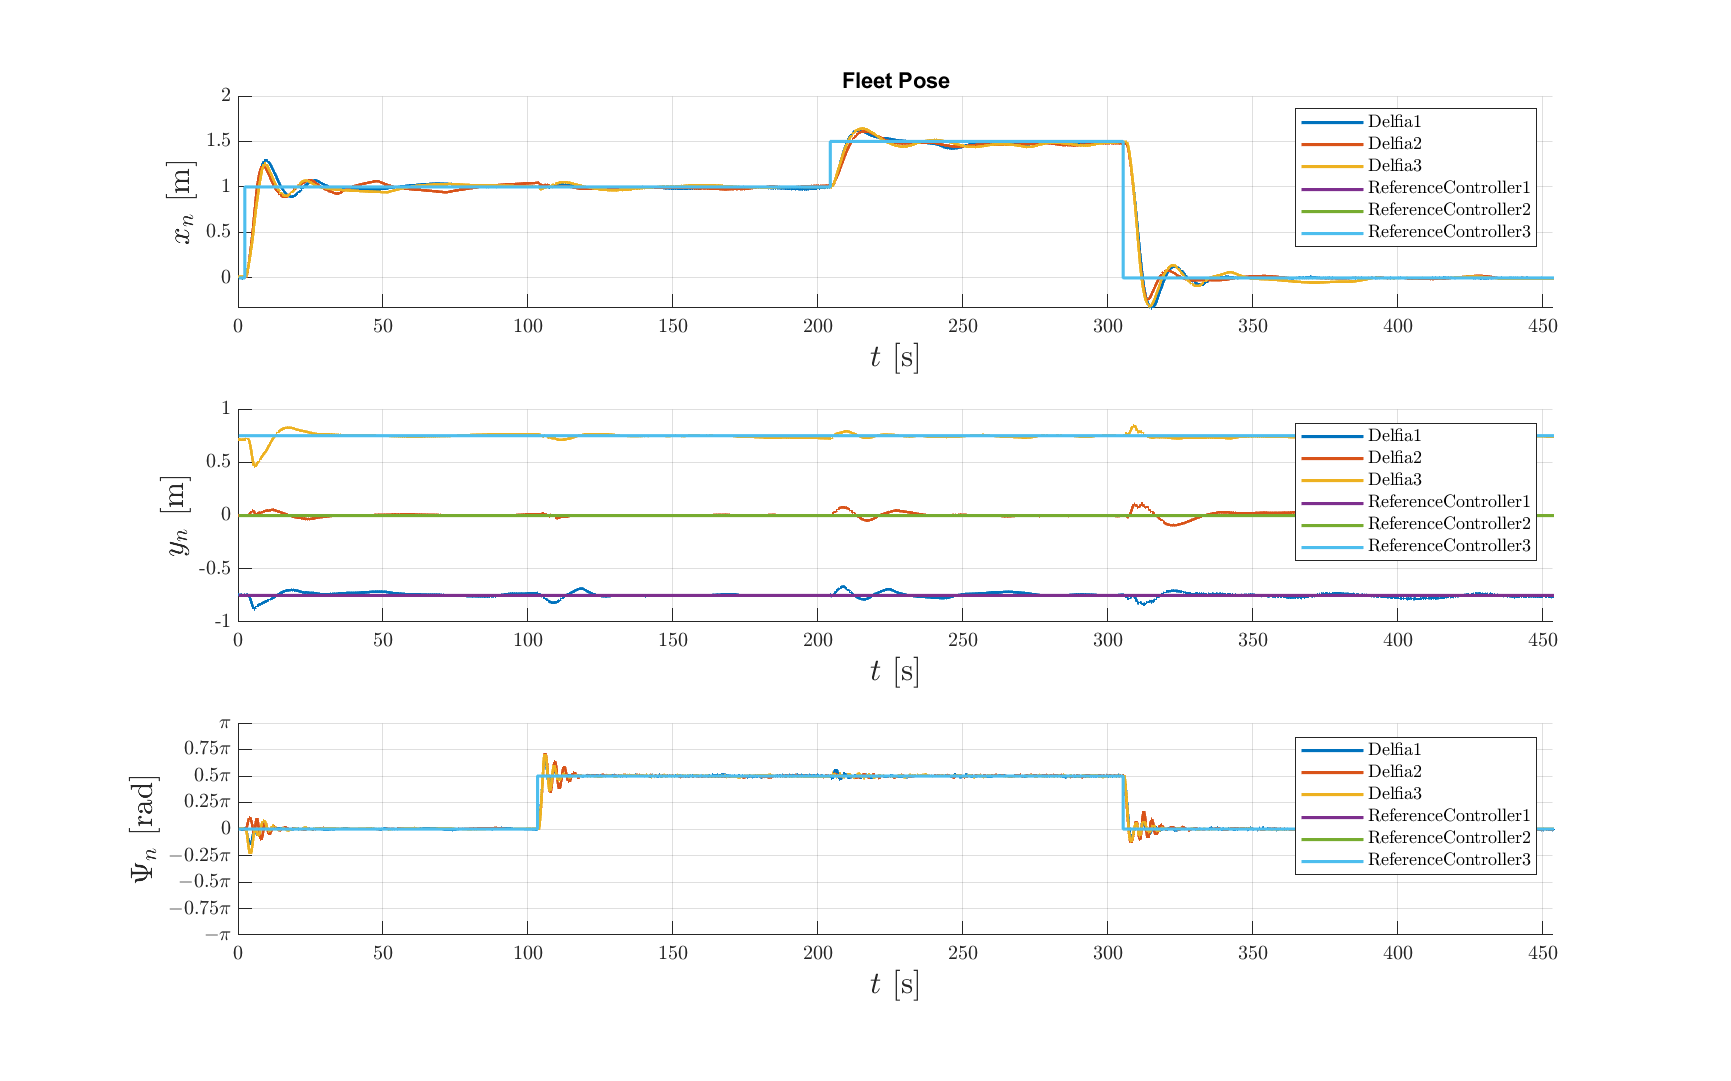
\includegraphics[width=1.0\textwidth]{matlabEvaluationFig18a.eps}
	\caption{3 separate vessels doing the similar step responses, but at an y-offset, such that they are besides oneanother. Three different step responses are done in this test representing forward, rotational and sideways motion.}
	\label{stepXYYAW1example}
\end{figure}

Throughout the process of iteratively improving control performance by adjusting gains, various insights were gained. 
A steady state error for all step responses was neglectably small without utilizing any integral control. This can be explained by the fact that the test setup was in a lab setting with little to no disturbances such as wind, current or waves. Thus there was no nessecity of setting any integral gain.
Dampening that was naturally present on the vessels proved to be quite significant without addition of derivative control. This is obviously thanks to hydrodynamic dampening. Enough dampening was considered to be naturally present in translation, and addition of more dampening terms only decreased performance. However, rotational motion did benefit from derivative control, as way more oscillation could be noticed in the responses. Magnitude of derivative gain for rotational motion formed as a balance between rise-time and settling-time. 

Hence the control gain tuning process formed control gains from the reference configuration. Following the control-gain scaling approach as described in section \ref{controlEffortGenerationDesign}, the configuration-independent control gains were set as follows
\begin{table}[H]
	\centering
\begin{tabular}{llll}
Dimention & Proportional gain & Integrator gain & Derivative gain \\
	\hline & & & \\[-5pt]
	translation $x$ and $y$ 	& $1.0$ $[m^{-1}]$		& $0$ $[s*m^{-1}]$ &  $0$  $[s^{-1}m^{-1}]$\\[3pt] 
	rotation $\Psi$ 			& $0.4456$ $[rad^{-1}]$			& $0$ $[s*rad^{-1}]$ & $0.15$ $[s^{-1}rad^{-1}]$\\ 
	\hline 
\end{tabular}
\caption{Configuration independent control gains that resulted from iterative system response evaluation and tuning.}
\end{table}

%\subsubsection{Adjustments on the assembly protocol}
The initial assembly protocol has been slightly adjusted throughout initial experiments. Early tests on platform assembly proved unable to perform within a reasonable timeframe. This was caused due to the fact that the magnet connectors did not reliably come into the area of acceptance upon which they would connect. Magnets seemed an attractive solution to connecting, especially as there was not a required approach direction during connecting, but vessels simply had to be adequately close to oneanother. Practically, modules would indeed be positioned in assembly orientation, yet oscillate a little, and not properly coming into contact. The area of acceptance proved too small for timely assembly with the current approach. The difficulties during connecting are visible in one test in particular, for which the module references and responses are shown in figure \ref{tp8_connecting_overall}. During this test the assembly protocol ran as described in section \ref{assemblyProtocolDesign} and illustrated in figure \ref{fig:matlabEvaluationFig14c}.

\begin{figure}[H]
	\centering
	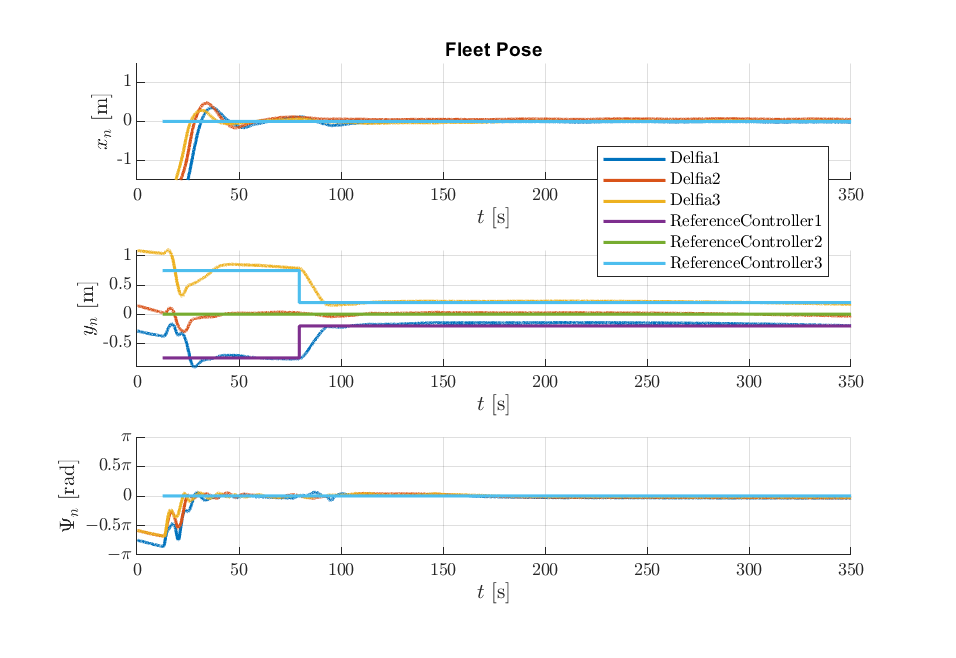
\includegraphics[width=1.0\textwidth]{tp8_connecting_overallb.eps}
	\caption{System responses during early connecting protocol. Notice how $x$ and $yaw$ reference remains constant. Most notably is the change in $y$ reference at $t=80s$. Assembly preparation and initial line-up occurs until this moment, after which the reference changes such that the vessels move to connection position.}
	\label{tp8_connecting_overall}
\end{figure}

From approximately $t=100$ one would expect modules to be approximately lined up such that magnet connectors could properly function. Successful connection can be judged in a more quantitative manner by expressing relative motion between modules. Succesful connections between modules should display zero or near zero relative motion. Figure \ref{tp8_connecting_relative_wide} \ref{AsseblyFailedRelative} show relative position between modules. For this, the body fixed frame of the middle vessel (module 2) is used, in which position of the connecting vessels (1 \& 3) are expressed (see figure \ref{fig:localframeShowing} for an illustration on how to interpret expressing location of a module in another vessel's body fixed coordinate system). 

\begin{figure}[H]
	\centering
	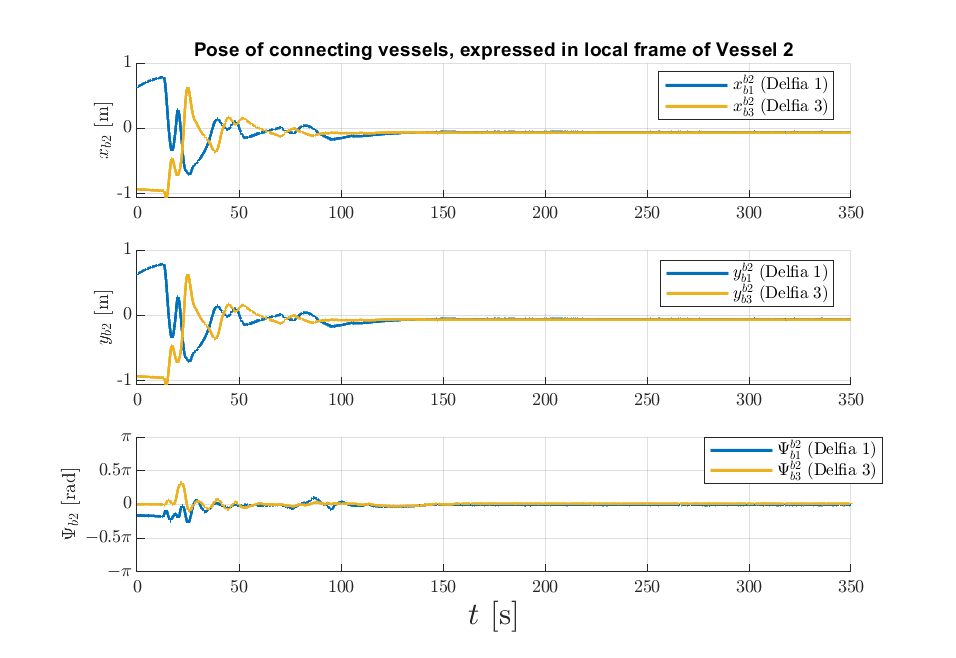
\includegraphics[width=0.9\textwidth]{tp8_connecting_relative_wide.eps}
	\caption{Relative motion of two modules connecting to module nr. 2, while running early assembly protocols.}
	\label{tp8_connecting_relative_wide}
\end{figure}

\begin{figure}[H]
	\centering
	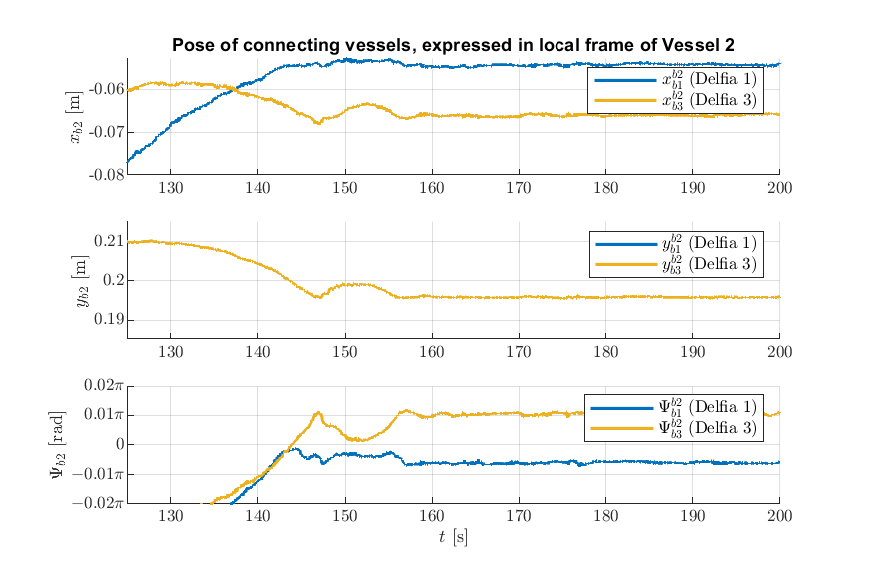
\includegraphics[width=0.9\textwidth]{tp8_connecting_relative_Zoomed.eps}
	\caption{Relative motion of two modules connecting to module nr. 2, while running early assembly protocols. Relative motion of a module stops in all three degrees of freedom, more or less at the same time, indicating succesful connection.}
	\label{AsseblyFailedRelative}
\end{figure}

Although connection was succesfully achieved, it required a period in the order of 70 seconds, which was considered rather long, even for a proof of concept. It was observed that modules were positioned near the connection site, but with lacking stimulants to get connectors into area of acceptance. Figure \ref{tp8_connecting_relative_state130t} illustrates how modules float around the connection site, while they were unconstrained in three degrees of motion, resulting in discrepancy in x y and yaw positioning.  Small errors in the definition of the body-fixed frame of the modules obtained from the optical tracking system, can be seen in figure \ref{AsseblyFailedRelative} and \ref{tp8_connecting_relative_state130t}, as the former shows nonzero $x$ and $\Psi$ values after connecting and the latter shows a seeming overlap of vessels. Relative motion in three degrees of freedom are present, which causes the modules to be misaligned, making succesful connecting less probable. Seeming overlap of module 1 \& 2 is caused by small errors in the definition of modules' origins. The definitions of the module's origins with respect to the optical trackers were slightly adjusted to decrease the magnitude of these errors for further tests. 

\begin{figure}[H]
	\centering
	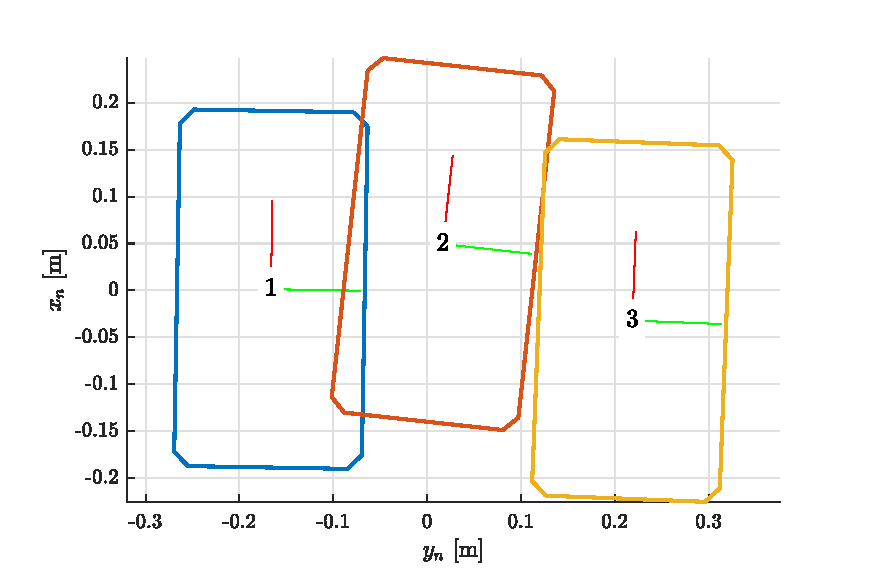
\includegraphics[width=0.7\textwidth]{tp8_connecting_relative_state130t.eps}
	\caption{Measured system state at $t=130s$ during early assembly test shown in figure \ref{tp8_connecting_relative_wide} and \ref{AsseblyFailedRelative}.}
	\label{tp8_connecting_relative_state130t}
\end{figure}
The problem of being insufficiently able to position modules within connector area of acceptance was solved by using normal forces on the modules' hulls to align surfaces. This is a common trick used by regular, human operated ships. A characteristic example is a ferry that pushes itself to a dock, such that it does not rotate or move, allowing safe transfer of passengers. A small normal force between vessels ensures that they keep making contact, and avoid rotation. As modules made contact, only one motion remained, which was translation along the contact surface. With only one degree of (relative) motion connections could be made timely. Figure \ref{DelfiasNormalForceIntoPush2} shows how normal forces have been created by setting contoller reference somewhat within the rigid body of a neighbouring module. Figure \ref{tp8_connecting_relative_wide} shows relative motion between modules of an assembling system that apply this approach. Notice that relative rotation and motion perpendicular to the contact surface are constrained first. Sliding motion along contact surface later stops as connectors snap into place. 

 \begin{figure}[H]
	\centering
	\makebox[\textwidth][c]{
		\begin{minipage}{0.47\textwidth}
			\centering
			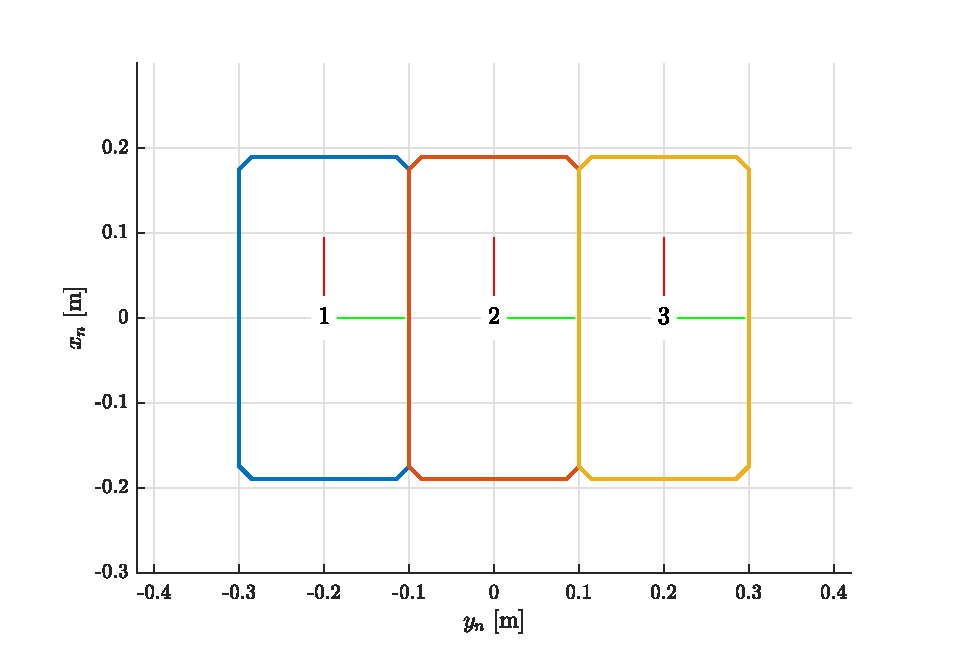
\includegraphics[width=1\textwidth]{img/3x1ConfigurationRef}
			\caption{Initial reference positions of modules for assembly}
			\label{3x1ConfigurationRef}
		\end{minipage}\hfill
		\begin{minipage}{0.45\textwidth}
			\centering
			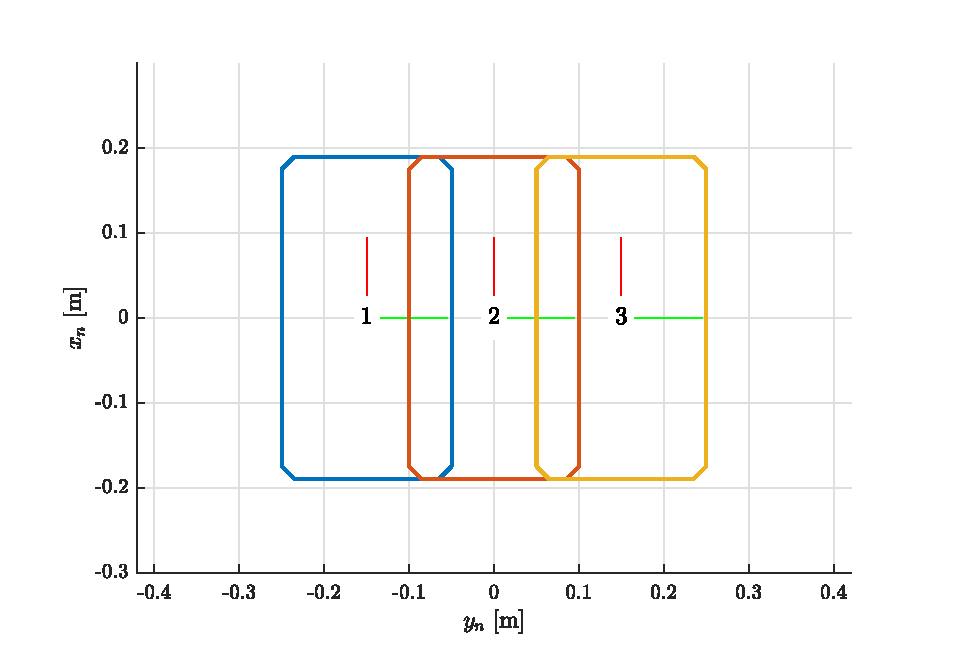
\includegraphics[width=1\textwidth]{img/3x1ConfigurationRef_overlapping}
			\caption{Adjusted references for positioning of modules while connecting, to create some normal forces between hulls. The shown references are impossible for the system to reach, as vessels are constrained by their hulls which can not overlap.}
			\label{3x1ConfigurationRef_overlapping}
		\end{minipage}
	}
\end{figure}

\begin{figure}[H]
	\centering
	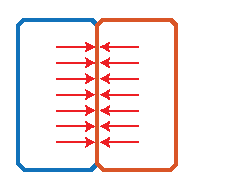
\includegraphics[width=0.4\textwidth]{VesselConnectTopvieuwReference_early.eps}
	\caption{Normal forces that result from overlapping references during assembly.}
	\label{DelfiasNormalForceIntoPush2}
\end{figure}

The normal forces between modules were kept to a minimum, as they purely function to remove motion between vessels perpendicular to the connection surface ($y$), and rotation. Remaining motion was by sliding along the connecting surface of the hull ($x$ direction), where friction did not seem to play a significant role with a smooth surface and low normal forces. 



\vspace{15mm}

This chapter explained design choices that characterize the developed self-assembling and cooperative fleet control system. At first, the multi-robot control approach with variable topology is explained after which the design of each subsystem is discussed. Implementation is thereafter explained, showing the realization of the fleet control system. The next chapter will assess performance of the  developed framework, to see whether or not the system performs according to the presented design criteria and goals. 

